\documentclass[runningheads]{llncs}
\usepackage[T1]{fontenc}
\usepackage{graphicx}
\usepackage{amsmath}
\usepackage{amssymb}
\usepackage{algorithm}
\usepackage{algpseudocode}
\usepackage{enumitem}
\usepackage{subcaption}
\usepackage{url}

% Ensure \doi and \arxiv exist even if llncs.cls does not define them.
\providecommand{\doi}[1]{\url{https://doi.org/#1}}
\providecommand{\arxiv}[1]{\url{https://arxiv.org/abs/#1}}

\setlength{\textfloatsep}{6pt plus 1pt minus 2pt}
\setlength{\floatsep}{6pt plus 1pt minus 2pt}
\setlength{\intextsep}{6pt plus 1pt minus 2pt}

\begin{document}
%
\title{SensitiveAI: A Hybrid AI System for Sensitive Content Detection and Moderation in Vietnamese}
\titlerunning{SensitiveAI: Hybrid Sensitive Content Detection and Moderation in Vietnamese}
%
\author{Pham Kha Vy\inst{1} \and Cao Hong Nga\inst{1}}
%
\authorrunning{P. K. Vy and C. H. Nga}
%
\institute{FPT University, Can Tho, Vietnam\\
\email{vypkce182254@fpt.edu.vn}\\
\email{caohongnga@gmail.com}}

%
\maketitle
%
\begin{abstract}
Automated content moderation is critical for maintaining safe online environments on social media platforms, forums, and messaging systems.
This paper presents \textbf{SensitiveAI}, a hybrid artificial intelligence system designed to detect and moderate sensitive content in Vietnamese.
The system integrates a \textit{rule-based detection engine} with a \textit{transformer-based deep learning model} (\texttt{mdeberta-v3-base}) to detect toxic, hateful, sexual, violent, and obfuscated content.
The rule engine combines normalized keyword matching across 16 weighted categories, regular-expression detection of personally identifiable information (PII), and specialized obfuscation detectors for leetspeak, homoglyphs, zero-width characters, Unicode mathematical fonts, and repeated or split characters.
The deep learning component uses a custom multi-label classification head with label-conditioned attention pooling, trained with a two-stage freeze-then-finetune protocol and discriminative learning rates.
On a Vietnamese subset of $17{,}367$ deduplicated training samples, the proposed configuration reaches a micro F1-score of $0.682$ (precision $0.692$, recall $0.674$, ROC-AUC $0.945$), an absolute improvement of $+4.6$ F1 points over standard fine-tuning evaluated at a fixed $0.5$ threshold (F1 $0.636$), with per-label threshold optimization contributing an additional $+0.2$ points on the same model.
Because only two of the six labels carry positive training examples, the multi-label head is currently evaluated on those two labels; the remaining four labels are retained in the architecture for when positive training data becomes available.
The rule engine and the neural model are fused by a \textit{max-score} policy with a high-confidence AI override: on the Vietnamese test set the fused system escalates $75.0\%$ of sensitive comments to \texttt{review}/\texttt{block} (versus $68.6\%$ for the model alone) while maintaining high coverage under automatic character-level obfuscation.

\keywords{content moderation \and hate speech detection \and hybrid AI \and transformer \and Vietnamese NLP}
\end{abstract}
%
\section{Introduction}

The rapid growth of online platforms has created unprecedented challenges in content moderation.
User-generated content---ranging from social media posts to forum comments and live chat messages---can contain toxic language, hate speech, threats, sexual content, and other forms of sensitive material that harm community standards and user well-being~\cite{zampieri2019}.

Traditional content moderation relies heavily on manual review, which is labor-intensive and psychologically taxing for moderators~\cite{roberts2019}, and commercial platforms increasingly turn to automation to handle the volume of content at scale~\cite{gorwa2020}.
Automated approaches that detect such content by inspecting the text itself have been studied extensively for English~\cite{warner2012,schmidt2017,wulczyn2017,devlin2019} and, to a lesser degree, for Vietnamese~\cite{luu2021,nguyen2020phobert}.
Yet robust Vietnamese-specific moderation still faces several open challenges:

\begin{enumerate}[leftmargin=*,label=(\roman*)]
\item \textbf{Vietnamese linguistic complexity:} Vietnamese is a tonal language with complex diacritical marks, creating unique challenges for text normalization and obfuscation detection.
\item \textbf{Obfuscation evasion:} users deliberately obfuscate sensitive words using character substitution, Unicode manipulation, zero-width characters, and creative spelling~\cite{cooper2023,boucher2022,mishra2018}.
\item \textbf{Context sensitivity:} accurate detection requires understanding semantic context, not just surface-level keyword matching.
\item \textbf{Class imbalance:} sensitive content is rare relative to benign content, so standard classifiers trained on the majority class perform poorly on minority categories~\cite{hegarcia2009}.
\end{enumerate}

This paper presents \textbf{SensitiveAI}, a hybrid content moderation system designed for Vietnamese.
Our approach combines the speed and interpretability of rule-based detection with the contextual understanding of a multilingual transformer.

The contributions of this work are:
\begin{itemize}[leftmargin=*]
\item A rule-based engine that matches sensitive keywords over normalized and diacritic-stripped text, scores them with category weights, and augments the score with an obfuscation bonus and a multi-category bonus, plus a PII regex layer and six obfuscation detectors.
\item A custom transformer head that pools the encoder output (CLS, mean, max) and uses label-conditioned multi-head attention over per-label query vectors.
\item A two-stage training protocol that freezes the encoder for the first 30\% of training steps and then fine-tunes all layers, combined with discriminative learning rates (linear ramp from 0.1\texttimes to 1.0\texttimes of the base learning rate).
\item An evaluation on a Vietnamese test split of $2{,}369$ samples and a validation split of $2{,}352$ samples from the cleaned corpus, with the reported checkpoints trained on the $17{,}367$-sample Vietnamese training split of a deduplicated corpus rebuild; four model configurations are compared on the same held-out test set, together with per-label threshold optimization.
\end{itemize}

\section{Related Work}
\label{sec:related}

\subsection{Automated Content Moderation}

Early automatic detection of abusive language used shallow features and classical classifiers: Warner and Hirschberg~\cite{warner2012} framed hate speech detection as word-sense disambiguation over n-grams with an SVM, and Schmidt and Wiegand~\cite{schmidt2017} survey the feature families used in subsequent work.
Wulczyn et al.~\cite{wulczyn2017} showed how crowdsourced labels combined with a trained classifier can scale personal-attack detection over Wikipedia comments.
More recently, pre-trained language models such as BERT~\cite{devlin2019} and domain-adapted variants such as HateBERT~\cite{caselli2021} became the dominant approach, and shared tasks such as OffensEval~\cite{zampieri2019} provide standardized benchmarks; Detoxify~\cite{hanu2020} is a widely used open toxic-text classifier.
Gorwa et al.~\cite{gorwa2020} discuss the technical and political challenges of \emph{algorithmic} content moderation, which motivates hybrid designs that combine transparent rules with learned models.

\subsection{Vietnamese Content Moderation}

Vietnamese presents unique challenges for moderation because of its tonal and diacritical writing system and frequent code-mixing.
The ViHSD corpus introduced by Luu et al.~\cite{luu2021} is the most widely used Vietnamese hate-speech benchmark.
Monolingual PhoBERT~\cite{nguyen2020phobert} and multilingual XLM-RoBERTa~\cite{conneau2020} and mDeBERTa~\cite{he2021deberta,he2023debertav3} have enabled transfer learning for Vietnamese NLP, including hate speech detection.

\subsection{Obfuscation and Evasion}

Users evade keyword filters by substituting letters (leetspeak, homoglyphs from different Unicode blocks), inserting zero-width characters, or spacing out words.
Cooper et al.~\cite{cooper2023} collected real-world English tweets in which hate words are masked with homoglyphs and showed that normalization substantially improves transformer-based detection.
Mishra et al.~\cite{mishra2018} propose character-based neural models that are robust to such obfuscation at the character level, and Boucher et al.~\cite{boucher2022} demonstrate imperceptible adversarial character perturbations that break NLP classifiers, motivating the normalization and obfuscation pipeline adopted in this paper.

\section{Methodology}
\label{sec:method}

\subsection{System Architecture Overview}

SensitiveAI processes each input as follows (see Fig.~\ref{fig:architecture}).
User input first passes through the \textbf{Text Normalization} module, which produces a normalized form for the rule engine; the AI model receives the raw text.
The normalized text is then analyzed by the \textbf{Rule Engine}, and the raw text by the \textbf{AI Transformer Model}.
A \textbf{Hybrid Decision} module fuses the rule-engine score and the model confidence into a final moderation decision.

\begin{figure}
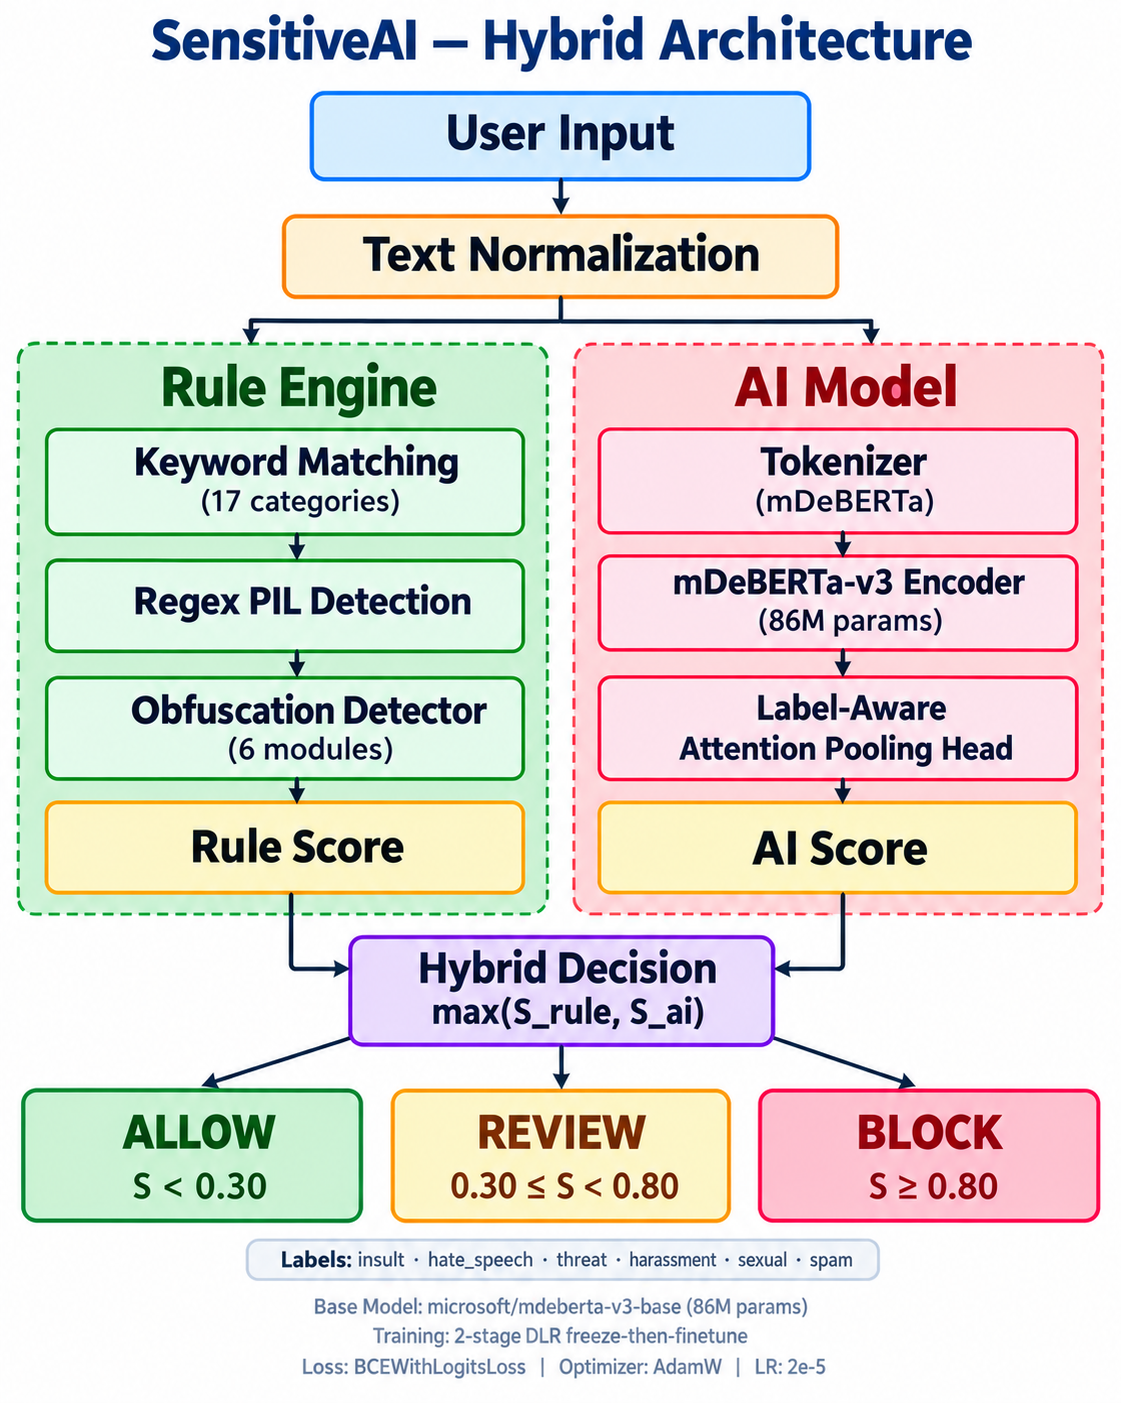
\includegraphics[width=\textwidth]{figures/architecture.png}
\caption{SensitiveAI hybrid architecture. Input is normalized for the rule engine, processed by the AI model in parallel, and the hybrid decision combines both signals to produce the final moderation action.}
\label{fig:architecture}
\end{figure}

\subsection{Text Normalization}

The normalization pipeline transforms raw text as follows (in execution order):
The normalization pipeline is applied in execution order: (1) Unicode NFKC normalization; (2) lowercasing; (3) temporary protection of e-mail, URL, phone, IP, and long-digit PII tokens; (4) removal of zero-width/control characters; (5) homoglyph normalization; (6) leetspeak normalization; (7) Vietnamese abbreviation expansion; (8) collapsing repetitions of length $\geq 3$; (9) special-character cleaning; (10) whitespace collapsing; (11) restoration of protected tokens; and (12) creation of a diacritic-stripped NFD variant used as a fallback by the rule engine.

The AI model is \emph{not} given the normalized text; it operates on the raw input so that the model can learn its own representations directly from raw text while the rule engine benefits from normalization.

\subsection{Rule Engine}

The rule engine combines three components: keyword matching, regex-based PII detection, and obfuscation detection.

\subsubsection{Keyword Matching.}
A curated dictionary of sensitive keywords is organized into 16 weighted categories, each with a severity weight (Table~\ref{tab:categories}).
Matching is performed on the normalized text (and, as a fallback, on the diacritic-stripped variant) with word-boundary, case-insensitive regular expressions.
Keywords in a whitelist are ignored, matches are greedily reserved longest-first and are not allowed to overlap, and each match carries a confidence that decreases with keyword length (1.0 for $\geq 12$, 0.95 for $\geq 8$, 0.90 for $\geq 5$, 0.85 otherwise).

\begin{table}
\centering\footnotesize
\caption{Keyword category weights used by the rule engine}\label{tab:categories}
\begin{tabular}{@{}llll@{}}
\hline
\textbf{Category} & \textbf{Weight} & \textbf{Category} & \textbf{Weight} \\
\hline
terrorism & 1.00 & gamble & 0.60 \\
sexual & 0.95 & religion & 0.50 \\
\shortstack{violence, self\_harm,\\ threat, hate\_speech,\\ racism} & 0.90 & politics & 0.40 \\
scam & 0.85 & \shortstack{profanity\_vi,\\ profanity\_en} & 0.65 \\
weapon, crime, drugs & 0.80 & & \\
\hline
\end{tabular}
\end{table}

\subsubsection{Scoring.}
Let $C_{\mathrm{matched}}$ be the set of matched categories and $w_c$ the weight of category $c$.
Let $\mathbf{1}_{\mathrm{obf}}$ indicate that an obfuscation technique was detected in the text.
The rule score is computed as
\begin{equation}
\label{eq:rule}
\begin{aligned}
S_{\mathrm{rule}} = &\min\Bigl(\; \max_{c \in C_{\mathrm{matched}}} w_c + 0.05 \cdot \mathbf{1}_{\mathrm{obf}} \\
&+ \min\bigl(0.05 \cdot \max(\lvert C_{\mathrm{matched}}\rvert - 1,\, 0),\; 0.15\bigr),\;\; 1.0 \Bigr),
\end{aligned}
\end{equation}
with $S_{\mathrm{rule}} = 0$ when no keyword matches.
The obfuscation bonus ($+0.05$) penalizes evasion attempts, and the multi-category bonus (capped at $+0.15$) reflects that several independent indicators are present.

The rule engine maps scores to a decision and a risk level as follows: score $0 \Rightarrow$ \texttt{allow} / \texttt{safe}; $0 < S < 0.60 \Rightarrow$ \texttt{flag} (risk \texttt{low} or \texttt{medium}); $0.60 \le S < 0.90 \Rightarrow$ \texttt{review} (risk up to \texttt{high}); $S \ge 0.90 \Rightarrow$ \texttt{block} (risk \texttt{critical}).
These thresholds are exactly those in \texttt{src/rules/rule\_engine.py}.

\subsubsection{Regex-Based PII Detection.}
Regular expressions detect: e-mail addresses, Vietnamese phone numbers, URLs, IPv4 addresses, credit-card-length digit sequences (13--19 digits), national-ID (CCCD) sequences (12 digits), bank-account-length sequences (9--16 digits), Bitcoin/Ethereum wallet identifiers, and social handles (Telegram, Discord, Facebook, Instagram, YouTube, TikTok, Zalo).
In the current implementation these matches are reported and counted in the moderation report, but they do \emph{not} change $S_{\mathrm{rule}}$ or the decision; whether PII evidence should force a hard \texttt{review}/\texttt{block} is a policy choice left to future work.

\subsubsection{Obfuscation Detection.}
Six regex detectors flag evasion techniques: split letters (word characters interleaved with spaces/other characters), leetspeak, mixed symbols, Unicode mathematical alphanumerics (U+1D400--U+1D7FF), zero-width characters, and repeated characters.
In addition, the normalization module reports whether homoglyph, leetspeak, abbreviation, zero-width, or repeated-character transformations were applied, and the \texttt{had\_*} metadata is fed back into the rule engine.
Detecting these strategies is important because keyword matching alone fails on obfuscated text~\cite{cooper2023,mishra2018,boucher2022}.

\subsection{AI Model}

\subsubsection{Base Model.}
We use \texttt{microsoft/mdeberta-v3-base} as the backbone, a multilingual DeBERTa variant pre-trained on 100 languages~\cite{he2023debertav3} that produces 768-dimensional contextual embeddings ($\approx$279M parameters, of which $\approx$193M are the 251k-token embedding and relative-position parameters; the encoder itself contributes $\approx$86M).

\subsubsection{Label-Conditioned Attention Pooling Head.}
Instead of classifying with a single linear layer over the CLS token, we use a custom head that pools the encoder output and refines $K=6$ per-label representations: it concatenates CLS, mean-pooled, and max-pooled representations ($2304$ dimensions), applies two 768-dimensional Dense--GELU--LayerNorm--Dropout blocks, projects to $K=6$ label-specific query vectors, adds learned label-position embeddings, applies 4-head self-attention among the label queries ($Q=K=V$), and uses residual normalization and one scalar logit per label.

The multi-label nature of the task (a comment may simultaneously be an insult and hate speech) is captured by the per-label logits, which are passed through independent sigmoids.



Because only two of the six labels have positive training examples in the Vietnamese split (see Sect.~\ref{sec:dataset}), the head is over-provisioned for the current data; the remaining label slots receive no supervision and, matching the absence of positive examples, produce no positive prediction at evaluation. We retain the $K=6$ design so that new labels only require new data, not an architectural change.

\subsubsection{Training Strategy.}
Two mechanisms are combined:

\textit{Two-stage freeze-then-finetune.} For the first \texttt{two\_stage\_freeze\_fraction}=0.3 (30\%) of all training steps the encoder is frozen and only the head is trained, so the randomly initialized head learns stable features before the encoder starts moving. At the switch point the whole model is fine-tuned for the remaining steps in a single continuous training run. The head (\texttt{head.*}/\texttt{classifier.*}/\texttt{score.*}) is trained in both stages.

\textit{Discriminative learning rates (DLR).} The encoder layers are assigned learning rates that ramp linearly from $0.1 \times \eta_{\mathrm{base}}$ (deepest layers and embeddings) to $1.0 \times \eta_{\mathrm{base}}$ (top layers); the classification head always receives the full $\eta_{\mathrm{base}}$. No separate head learning rate is configured in the reported runs.

\subsubsection{Loss and Imbalance Handling.}
The model is trained with binary cross-entropy with logits (BCEWithLogitsLoss) over the $K$ labels. Class weights (pos-weight for hate\_speech $= 2.0$) and focal loss are implemented in the codebase (\texttt{src/training/trainer.py}) but were disabled in the runs that produced the reported results.

\subsubsection{Per-Label Threshold Optimization.}
Instead of a single threshold of 0.5 for all labels, per-label thresholds $\tau_k$ are selected on the validation set by grid search, maximizing either $F_1$ or $F_2$ under a minimum-precision constraint $P \ge 0.5$, a strategy common in multi-label classification~\cite{tsoumakas2007}. The selected thresholds are then used at test time. Table~\ref{tab:threshold} reports the effect of this choice.

\subsection{Hybrid Decision Mechanism}

The final moderation score combines rule-based and AI-based signals. The AI confidence $S_{\mathrm{ai}}$ is the largest sigmoid score among the labels flagged as present at the runtime threshold ($0.5$):
\begin{equation}
\label{eq:fusion}
S_{\mathrm{final}} = \max(S_{\mathrm{rule}},\ S_{\mathrm{ai}}),
\end{equation}
and the rule-engine decision (\texttt{allow}/\texttt{flag}/\texttt{review}/\texttt{block} per Sect.~\ref{sec:method}) is taken initially.

A high-confidence AI override tightens the rule-based decision for very confident predictions:
\begin{itemize}[leftmargin=*]
\item if $S_{\mathrm{ai}} \ge 0.95$ the decision is forced to \texttt{block} (risk \texttt{critical});
\item if $0.80 \le S_{\mathrm{ai}} < 0.95$ an existing \texttt{allow} becomes \texttt{review}, and a \texttt{safe}/\texttt{low} risk becomes \texttt{high}.
\end{itemize}

The final category set and the \emph{sensitive} flag are the unions of the rule-engine and model outputs. A sensitivity plan therefore fuses both signals.

We reconcile the two threshold regimes explicitly: the \emph{deployed runtime} applies the default label threshold ($0.5$) inside this policy, while the \emph{reported metrics of the proposed configuration} use its F1-optimized thresholds ($\tau_{\mathrm{insult}}=0.25$, $\tau_{\mathrm{hate\_speech}}=0.30$); the other configurations in Table~\ref{tab:results_vi} were archived at the fixed $0.5$ threshold. Under the deployed operating point the end-to-end hybrid (rules $+$ model $+$ overrides) escalates $75.0\%$ of the $440$ sensitive test comments (versus $68.6\%$ for the model alone and $43.2\%$ for the rule engine alone), passing $25.0\%$ as \texttt{allow}, at a cost of escalating $14.7\%$ of the $1{,}929$ clean comments---a precision--recall trade-off appropriate for a review-first workflow (Table~\ref{tab:fusion}).

\begin{table}
\caption{End-to-end behavior of the deployed policy on the full test set at the runtime $0.5$ operating point}\label{tab:fusion}
\centering
\footnotesize
\begin{tabular}{@{}lrrr@{}}
\hline
\textbf{Decision} & \textbf{Total} & \textbf{Sensitive} & \textbf{Clean} \\
\hline
ALLOW  & 1{,}755 & 110 & 1{,}645 \\
REVIEW &   209  &  54  &  155  \\
BLOCK  &   405  & 276  &  129  \\
\hline
\end{tabular}
\end{table}



\section{Experiments}
\label{sec:experiments}

\subsection{Dataset}
\label{sec:dataset}

We evaluate on a Vietnamese multilabel dataset with six toxic-content labels (insult, hate\_speech, threat, harassment, sexual, spam). The corpus is constructed from the label-mapped \texttt{uitnlp/vihsd} collection~\cite{luu2021} and the English Jigsaw toxic-comment collection~\cite{jigsaw2018} (mapped label-wise into the same schema), bilingual and filtered to language $=$ \texttt{vi}; the per-split counts below are from \texttt{dataset/clean/*.csv} and therefore do \emph{not} coincide with ViHSD's official split sizes.

The split contains positive examples only for \emph{insult} and \emph{hate\_speech}; the other four labels are all-negative in every split. Moreover, \emph{hate\_speech} is a strict subset of \emph{insult}, so the current six-label evaluation is effectively binary.

Table~\ref{tab:dataset} lists the per-split counts.

Two builds of the cleaned corpus are used in this study. Build \texttt{v1} (\texttt{dataset/clean/*.csv}, Table~\ref{tab:dataset}) provides the validation ($2{,}352$) and test ($2{,}369$) Vietnamese splits on which all reported metrics and threshold selections are computed. Build \texttt{v2} (\texttt{dataset/clean/v2}, Vietnamese subset \texttt{dataset/clean/v2\_vi}) is a rebuild of the same raw corpus that additionally enforces within- and cross-split deduplication of normalized texts (priority test $>$ validation $>$ train; duplicate rows are dropped, never moved); its Vietnamese splits contain $17{,}367/2{,}311/2{,}365$ train/validation/test samples with no cross-split duplicate of the normalized text. The reported checkpoints were trained on the \texttt{v2} Vietnamese training split ($17{,}367$) with early stopping on its validation split ($2{,}311$). The two builds come from separate passes over the same raw data, so the smaller \texttt{v2} training count is not obtained by deleting rows from the \texttt{v1} training column; the \texttt{v1} validation and test columns are exactly the splits used in every reported evaluation.

\begin{table}
\centering\footnotesize
\caption{Vietnamese dataset statistics (from \texttt{dataset/clean/*.csv}, language $=$ \texttt{vi})}\label{tab:dataset}
\begin{tabular}{@{}lrrrr@{}}
\hline
\textbf{Split} & \textbf{Total} & \textbf{Insult} & \textbf{Hate\_speech} & \textbf{Clean} \\
\hline
Train & 17,926 & 3,169 & 1,934 & 14,757 \\
Validation & 2,352 & 407 & 264 & 1,945 \\
Test & 2,369 & 440 & 289 & 1,929 \\
\hline
\end{tabular}
\end{table}

Additionally, a Vietnamese augmented training set of 30,066 rows was generated with six obfuscation-aware transformations (abbreviation substitution, homoglyph substitution, leetspeak substitution, random casing, special-character insertion, and zero-width insertion), sampling 2--5 random transformations per output, with 5 variants per hate\_speech sample and 2 per insult-only sample. The reported checkpoints were trained on the original non-augmented set; the augmented set is reserved for robustness training in future work.

\subsection{Training Configuration}

Hyperparameters are summarized in Table~\ref{tab:hyperparams}. All reported runs use the default random seed $42$; single-seed results are reported without significance testing.

\begin{table}
\centering\footnotesize
\caption{Hyperparameters}\label{tab:hyperparams}
\begin{tabular}{@{}ll@{}}
\hline
\textbf{Parameter} & \textbf{Value} \\
\hline
Base model & \texttt{mdeberta-v3-base} (multilingual, 768-d) \\
Max sequence length & 256 tokens \\
Per-device batch & 8 (gradient accumulation 4) \\
Optimizer & AdamW (default $\beta_1$=0.9, $\beta_2$=0.999) \\
LR scheduler & cosine, warmup ratio 0.1 \\
Base learning rate & $2\times10^{-5}$ \\
DLR & linear multiplier $0.1 \to 1.0$ over encoder layers; head $1.0$ \\
Two-stage & freeze encoder for first 30\% of steps \\
Epochs & 3 \\
Weight decay & 0.01 \\
Precision & FP16 \\
Loss & BCEWithLogitsLoss (multi-label) \\
Early stopping & patience 4, best model by validation F1 \\
Decision thresholds (proposed config.) & $\tau_{\mathrm{insult}}=0.25$, $\tau_{\mathrm{hate\_speech}}=0.30$ (others 0.5) \\
Random seed & 42 (default) \\
\hline
\end{tabular}
\end{table}

\subsection{Evaluation Metrics}

For multi-label evaluation we micro-average precision, recall, and F1 over all label--example pairs; \textbf{Accuracy} is the exact-match ratio (all six labels must match); \textbf{ROC-AUC} and \textbf{PR-AUC} are computed micro-averaged over the six binary problems from the sigmoid label probabilities (threshold-independent). Precision, recall, F1, and Accuracy use the per-class decision thresholds described below. Since the four labels without positives are predicted negative throughout, exact-match accuracy is effectively governed by the insult and hate\_speech predictions.

\subsection{Experimental Design}

We evaluate four real model checkpoints on the same $2{,}369$-instance Vietnamese test set. The archived evaluation of the first three configurations used the fixed $0.5$ threshold: \textbf{sensitiveai-vi} (standard fine-tuning of \texttt{mdeberta-v3-base} with a linear head), \textbf{sensitiveai-v1-vi} (standard head, the in-domain checkpoint from which the later models warm-start), and \textbf{sensitiveai-vi-custom-v2} (custom head, warm-started from \texttt{sensitiveai-v1-vi}). The proposed configuration, \textbf{sensitiveai-vi-custom-dlr2stage} (custom head with DLR and two-stage training, warm-started from \texttt{sensitiveai-v1-vi}), is evaluated at its F1-optimized per-class thresholds $0.25/0.30$; threshold optimization was performed only for this configuration (Table~\ref{tab:threshold}). An untrained baseline is omitted: an initial-weights model is seed-dependent and does not constitute a meaningful comparison point. Each configuration is a single training run; single-seed point estimates are reported without significance testing.

\subsection{Results}

Table~\ref{tab:results_vi} summarizes overall performance on the Vietnamese test set.

\begin{table}
\centering\footnotesize\setlength{\tabcolsep}{4pt}
\caption{Results on the Vietnamese test set (micro-averaged; the first three configurations evaluated at the fixed $0.5$ threshold, the proposed configuration at its F1-optimized per-class thresholds)}\label{tab:results_vi}
\begin{tabular}{@{}lcccccc@{}}
\hline
\textbf{Model} & \textbf{Acc} & \textbf{Prec} & \textbf{Rec} & \textbf{F1} & \textbf{ROC-AUC} & \textbf{PR-AUC} \\
\hline
sensitiveai-vi & 0.8569 & 0.7279 & 0.5652 & 0.6363 & 0.9688 & 0.7064 \\
sensitiveai-v1-vi & 0.8649 & 0.7145 & 0.6008 & 0.6528 & 0.9669 & 0.7136 \\
sensitiveai-vi-custom\newline v2 & 0.8662 & 0.6996 & 0.6612 & 0.6798 & 0.9617 & 0.6902 \\
\textbf{sensitiveai-vi-custom\newline dlr2stage} & \textbf{0.8658} & \textbf{0.6915} & \textbf{0.6735} & \textbf{0.6824} & \textbf{0.9453} & \textbf{0.6899} \\
\hline
\end{tabular}
\end{table}
\setlength{\tabcolsep}{6pt}

The proposed configuration (\textbf{sensitiveai-vi-custom-dlr2stage}) reaches the highest F1 of \textbf{0.6824}. Relative to standard fine-tuning evaluated at the fixed $0.5$ threshold (sensitiveai-vi, F1 $0.636$, recall $0.565$) this is a gain of $+4.6$ F1 points. The gain decomposes into warm-starting, the custom head, DLR + two-stage training, and threshold optimization: sensitiveai-v1-vi reaches F1 $0.653$, sensitiveai-vi-custom-v2 $0.680$ ($+2.7$ points from the custom head on top of warm-starting), DLR + two-stage add $\approx +0.3$ points, and per-label threshold optimization contributes another $\approx +0.2$ points (F1 $0.681$ at a fixed $0.5$ threshold on the proposed model). The proposed configuration has the \emph{lowest} ROC-AUC among the fine-tuned variants ($0.945$ vs.\ $0.962$--$0.969$) and trades a small amount of precision for recall, so the ``best model'' claim rests on the F1/system-level ordering at the selected operating points rather than on a uniform improvement.

Per-label results are given in Table~\ref{tab:per_label}. Because the four labels without positive examples have no positive instances, their precision, recall, and F1 are undefined; they are marked ``--'' in the table.

\begin{table}
\centering\footnotesize
\caption{Per-label results (\textit{sensitiveai-vi-custom-dlr2stage}); ``--'' denotes an undefined metric (label has no positive instances)}\label{tab:per_label}
\begin{tabular}{@{}lcccc@{}}
\hline
\textbf{Label} & \textbf{Prec} & \textbf{Rec} & \textbf{F1} & \textbf{Support} \\
\hline
insult & 0.716 & 0.711 & 0.714 & 440 \\
hate\_speech & 0.652 & 0.616 & 0.634 & 289 \\
threat & -- & -- & -- & 0 \\
harassment & -- & -- & -- & 0 \\
sexual & -- & -- & -- & 0 \\
spam & -- & -- & -- & 0 \\
\hline
\end{tabular}
\end{table}

\subsubsection{Confusion Matrices.}
Figure~\ref{fig:cm} presents the confusion matrices for the two labels with ground-truth data; Figures~\ref{fig:roc} and~\ref{fig:pr} present the corresponding ROC and precision--recall curves.

\begin{figure}
\centering
\begin{minipage}{.38\textwidth}
\centering
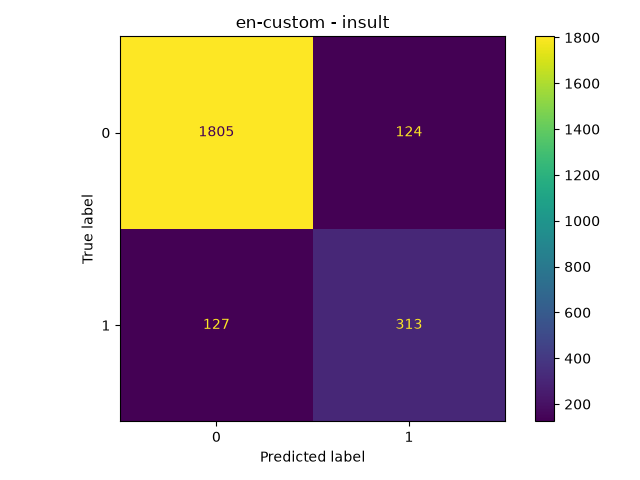
\includegraphics[width=\textwidth]{figures/confusion_matrix_insult.png}
\caption{Insult}
\label{fig:cm_insult}
\end{minipage}
\hfill
\begin{minipage}{.38\textwidth}
\centering
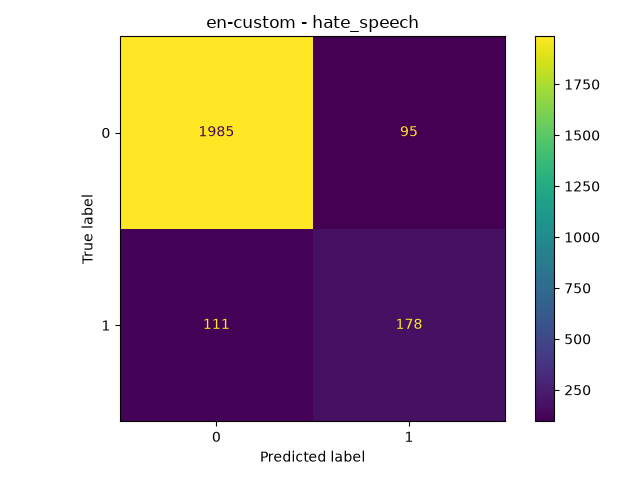
\includegraphics[width=\textwidth]{figures/confusion_matrix_hate_speech.png}
\caption{Hate speech}
\label{fig:cm_hate}
\end{minipage}
\caption{Confusion matrices on the Vietnamese test set}
\label{fig:cm}
\end{figure}

\subsubsection{ROC and PR Curves.}
Figures~\ref{fig:roc} and~\ref{fig:pr} present the ROC and precision--recall curves for each label.

\begin{figure}
\centering
\begin{minipage}{.38\textwidth}
\centering
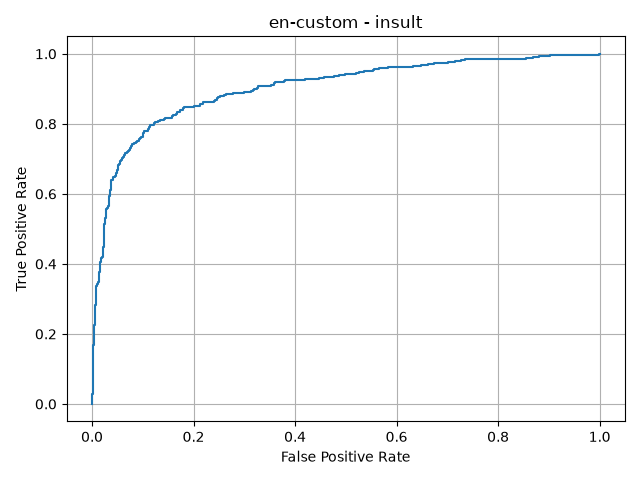
\includegraphics[width=\textwidth]{figures/roc_curve_insult.png}
\caption{Insult}
\label{fig:roc_insult}
\end{minipage}
\hfill
\begin{minipage}{.38\textwidth}
\centering
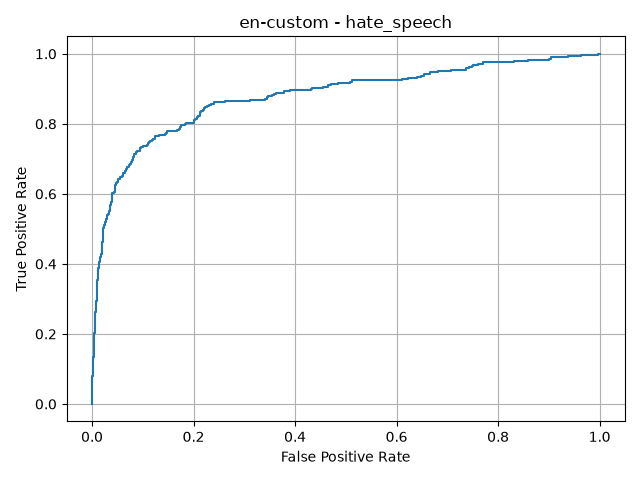
\includegraphics[width=\textwidth]{figures/roc_curve_hate_speech.png}
\caption{Hate speech}
\label{fig:roc_hate}
\end{minipage}
\caption{ROC curves on the Vietnamese test set}
\label{fig:roc}
\end{figure}

\begin{figure}
\centering
\begin{minipage}{.38\textwidth}
\centering
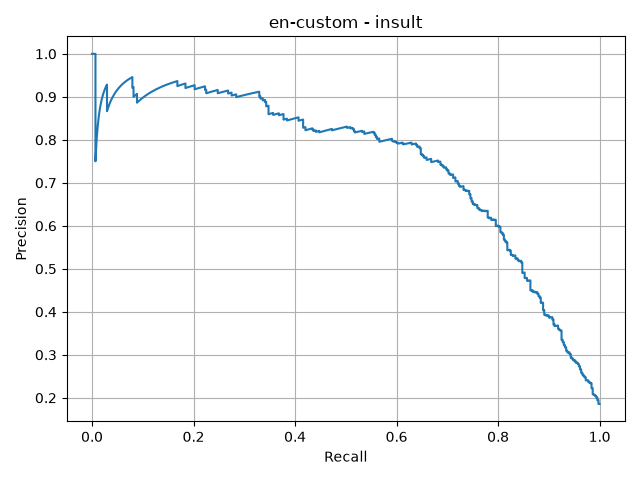
\includegraphics[width=\textwidth]{figures/pr_curve_insult.png}
\caption{Insult}
\label{fig:pr_insult}
\end{minipage}
\hfill
\begin{minipage}{.38\textwidth}
\centering
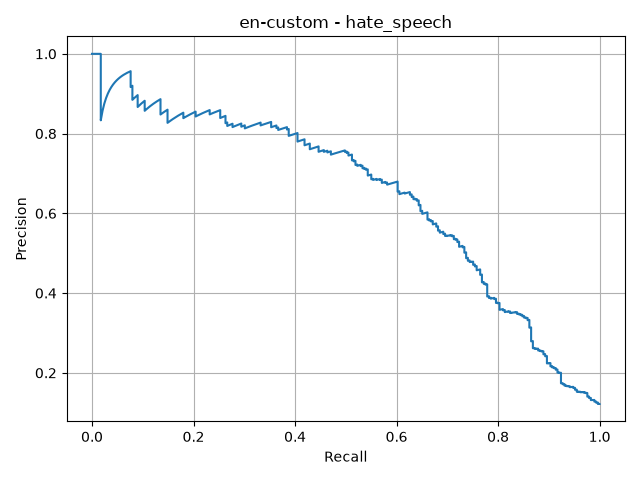
\includegraphics[width=\textwidth]{figures/pr_curve_hate_speech.png}
\caption{Hate speech}
\label{fig:pr_hate}
\end{minipage}
\caption{Precision--recall curves on the Vietnamese test set}
\label{fig:pr}
\end{figure}

\subsubsection{Threshold Optimization.}
Table~\ref{tab:threshold} shows the effect of per-label threshold optimization on the test set for the proposed configuration (thresholds selected on the validation split). The F1-optimized thresholds ($0.25/0.30$) are those used for the headline numbers in Table~\ref{tab:results_vi}; a fixed $0.5$ threshold loses $0.2$ points of F1, and a recall-oriented (F${}_2$) choice trades precision for about $+4.7$ points of recall.

\begin{table}
\centering\footnotesize
\caption{Threshold optimization results (\textit{sensitiveai-vi-custom-dlr2stage})}\label{tab:threshold}
\begin{tabular}{@{}lccc@{}}
\hline
\textbf{Configuration} & \textbf{Prec} & \textbf{Rec} & \textbf{F1} \\
\hline
Flat threshold $=$ 0.50 & 0.721 & 0.645 & 0.681 \\
Recall-oriented (F${}_2$, $\tau$=0.05/0.05) & 0.623 & 0.720 & 0.668 \\
F1-optimized ($\tau$=0.25/0.30) & 0.692 & 0.674 & 0.682 \\
\hline
\end{tabular}
\end{table}

\section{Discussion}
\label{sec:discussion}

\subsection{Effectiveness of the Training Strategy}

The proposed two-stage DLR configuration reaches the highest F1 in Table~\ref{tab:results_vi}. The freeze-then-finetune protocol lets the randomly initialized head learn stable label-specific features before the encoder is unfrozen, mitigating catastrophic forgetting on a small fine-tuning set~\cite{goodfellow2013}. The gain over the warm-started custom-head variant (F1 $0.680$) is small ($+0.3$ points) and the ROC-AUC ordering is reversed, so the improvement is not uniform across operating points: standard fine-tuning ($0.636$) improves to $0.653$ with warm-starting from the in-domain checkpoint and to $0.680$ once the custom head is added, while DLR and two-stage training add a further $+0.3$ points and shift the operating point toward higher recall. All differences are single-run point estimates rather than tested effects.

\subsection{Class Imbalance and the Multi-Label Setting}

Only two of the six labels have positives, and hate\_speech is a strict subset of insult, so the micro-averaged metrics largely measure the insult predictor: the reported $K=6$ system is effectively evaluated as a binary classifier. Annotating the remaining labels, or re-examining the redundant-label annotation, is required before a full multi-label evaluation.

\subsection{Obfuscation Detection}

The rule engine incorporates six obfuscation detectors plus a $+0.05$ score bonus for obfuscated content, mirroring real-world evasion~\cite{cooper2023,mishra2018,boucher2022}. A robustness evaluation on the $440$ sensitive test comments (each positive rewritten with automatic character-level perturbations) shows the fused pipeline retains most of its coverage: the rule engine alone flags $43.2\%$ of the original positives and stays at $43.0$--$43.2\%$ under every single technique; the raw-text model alone covers $68.9\%$ originally and $68.9$--$75.5\%$ under the conventional single techniques; the fused system (rules $\cup$ raw-text model) reaches $78.2\%$ on the original positives ($344/440$) and $77.7$--$83.4\%$ under conventional techniques, and the model and the fused system reach $77.3\%$ and $87.0\%$, respectively, when three techniques are combined. Zero-width insertion is distinctive: the raw-text model and the fused system retain $88.4\%$ and $93.0\%$, respectively, whereas the same inputs after normalization drop to $71.4\%$ because zero-width characters are stripped before keyword matching, so the raw-text path remains the primary defence; a tuned adaptive attack is left to future work.

\subsection{Limitations}

The main limitations are the label deficit and redundant hate\_speech/insult annotations; single-run evaluation without variance or significance tests; the hybrid demonstrated at a single operating point rather than a tuned orchestration; PII evidence not affecting decisions; the deliberate runtime/reported-threshold split; and the moderate performance ceiling of the current dataset.

\section{Conclusion and Future Work}

This paper presented SensitiveAI, a hybrid system for sensitive content detection in Vietnamese combining a normalization-aware rule engine (16 weighted keyword categories, PII regexes, six obfuscation detectors) with a multilingual transformer and a custom label-conditioned attention pooling head trained with two-stage freeze-then-finetune and discriminative learning rates. The two-stage DLR configuration reaches the highest F1 (0.682), a gain of $+4.6$ points over standard fine-tuning evaluated at a fixed $0.5$ threshold and $+0.3$~points over the warm-started custom-head configuration; warm-starting and the custom head deliver most of the gain, threshold optimization shifts the precision--recall operating point, and the fused rules+model system escalates $75.0\%$ of sensitive comments while retaining high coverage under automatic character-level obfuscation. The current data effectively evaluate only insult/hate\_speech while the remaining four head slots are unsupervised.

Future work: (1) tuning fusion thresholds and override levels and testing a tuned orchestration; (2) adversarial robustness ablations with adaptive obfuscation; (3) real positives for the remaining labels and re-annotation of the nested hate\_speech/insult relation; (4) PhoBERT and larger backbones; (5) repeated-seed variance reporting; and (6) explainability of the rule and attention-based head.

\begin{credits}
\subsubsection{\ackname}
This research was conducted as a Capstone Project at FPT University.

\subsubsection{\discintname}
The authors have no competing interests to declare that are relevant to the content of this article.
\end{credits}
%
% ---- Bibliography ----
% All entries below were verified against their venues/DOIs.
%
\begin{thebibliography}{99}

\bibitem{zampieri2019}
Zampieri, M., Malmasi, S., Nakov, P., Rosenthal, S., Farra, N., Kumar, R.: Predicting the type and target of offensive posts in social media. In: Proc.\ NAACL-HLT 2019, pp.~1415--1420. Association for Computational Linguistics (2019). \doi{10.18653/v1/N19-1144}

\bibitem{roberts2019}
Roberts, S.T.: Behind the Screen: Content Moderation in the Shadows of Social Media. Yale University Press (2019).

\bibitem{gorwa2020}
Gorwa, R., Binns, R., Katzenbach, C.: Algorithmic content moderation: Technical and political challenges in the automation of platform governance. Big Data \& Society \textbf{7}(1), 1--15 (2020).
\doi{10.1177/2053951719897945}

\bibitem{warner2012}
Warner, W., Hirschberg, J.: Detecting hate speech on the world wide web. In: Proc.\ Second Workshop on Language in Social Media (LSM), pp.~19--26 (2012).

\bibitem{schmidt2017}
Schmidt, A., Wiegand, M.: A survey on hate speech detection using natural language processing. In: Proc.\ Fifth International Workshop on Natural Language Processing for Social Media, pp.~1--10 (2017).

\bibitem{wulczyn2017}
Wulczyn, E., Thain, N., Dixon, L.: Ex machina: Personal attacks seen at scale. In: Proc.\ 26th International Conference on World Wide Web (WWW), pp.~1391--1399 (2017).
\doi{10.1145/3038912.3052591}

\bibitem{devlin2019}
Devlin, J., Chang, M.-W., Lee, K., Toutanova, K.: BERT: Pre-training of deep bidirectional transformers for language understanding. In: Proc.\ NAACL-HLT 2019, pp.~4171--4186 (2019).
\doi{10.18653/v1/N19-1423}

\bibitem{caselli2021}
Caselli, T., Basile, V., Mitrovi\'{c}, J., Granitzer, M.: HateBERT: Retraining BERT for abusive language detection in English. In: Proc.\ 5th Workshop on Online Abuse and Harms (WOAH), pp.~17--25 (2021).
\doi{10.18653/v1/2021.woah-1.3}

\bibitem{hanu2020}
Hanu, L., Unitary team: Detoxify: Toxic comment classification (2020). \url{https://github.com/unitaryai/detoxify}

\bibitem{luu2021}
Luu, S.T., Nguyen, K.V., Nguyen, N.L.-T.: A large-scale dataset for hate speech detection on Vietnamese social media texts. In: Proc.\ IEA/AIE 2021, LNCS vol.~12798, pp.~415--426. Springer (2021). \doi{10.1007/978-3-030-79457-6\_35}

\bibitem{nguyen2020phobert}
Nguyen, D.Q., Nguyen, A.T.: PhoBERT: Pre-trained language models for Vietnamese. In: Findings of EMNLP 2020, pp.~1037--1042 (2020).
\doi{10.18653/v1/2020.findings-emnlp.92}

\bibitem{conneau2020}
Conneau, A., Khandelwal, K., Goyal, N., Chaudhary, V., Wenzek, G., Guzm\'{a}n, F., Grave, E., Ott, M., Zettlemoyer, L., Stoyanov, V.: Unsupervised cross-lingual representation learning at scale. In: Proc.\ ACL 2020, pp.~8440--8451 (2020).
\doi{10.18653/v1/2020.acl-main.747}

\bibitem{he2021deberta}
He, P., Liu, X., Gao, J., Chen, W.: DeBERTa: Decoding-enhanced BERT with disentangled attention. In: Proc.\ ICLR 2021.

\bibitem{he2023debertav3}
He, P., Gao, J., Chen, W.: DeBERTaV3: Improving DeBERTa using ELECTRA-style pre-training with gradient-disentangled embedding sharing. In: Proc.\ ICLR 2023. \arxiv{2111.09543}

\bibitem{cooper2023}
Cooper, P., Surdeanu, M., Blanco, E.: Hiding in plain sight: Tweets with hate speech masked by homoglyphs. In: Findings of EMNLP 2023, pp.~2922--2929 (2023).
\doi{10.18653/v1/2023.findings-emnlp.192}

\bibitem{mishra2018}
Mishra, P., Yannakoudakis, H., Shutova, E.: Neural character-based composition models for abuse detection. In: Proc.\ 2nd Workshop on Abusive Language Online (ALW2) (2018). \arxiv{1809.03878}
\doi{10.18653/v1/W18-5101}

\bibitem{boucher2022}
Boucher, N., Shumailov, I., Anderson, R., Papernot, N.: Bad characters: Imperceptible NLP attacks. In: Proc.\ IEEE Symposium on Security and Privacy (S\&P) (2022). \arxiv{2106.09898}

\bibitem{hegarcia2009}
He, H., Garcia, E.A.: Learning from imbalanced data. IEEE Transactions on Knowledge and Data Engineering \textbf{21}(9), 1263--1284 (2009).
\doi{10.1109/TKDE.2008.239}

\bibitem{goodfellow2013}
Goodfellow, I.J., Mirza, M., Xiao, D., Courville, A., Bengio, Y.: An empirical investigation of catastrophic forgetting in gradient-based neural networks. arXiv:1312.6211 (2013).

\bibitem{tsoumakas2007}
Tsoumakas, G., Katakis, I.: Multi-label classification: An overview. International Journal of Data Warehousing and Mining \textbf{3}(3), 1--13 (2007).

\bibitem{vaswani2017}
Vaswani, A., Shazeer, N., Parmar, N., Uszkoreit, J., Jones, L., Gomez, A.N., Kaiser, \L., Polosukhin, I.: Attention is all you need. In: Advances in Neural Information Processing Systems 30 (NeurIPS), pp.~5998--6008 (2017).

\bibitem{jigsaw2018}
Conversation AIs: Unintended Bias in Toxicity Classification (Jigsaw Toxic Comment Classification Challenge). Kaggle (2018). \url{https://www.kaggle.com/c/jigsaw-toxic-comment-classification-challenge}

\end{thebibliography}
\end{document}'